\section{Empirical and Engine Verification}\label{sec:eval}
We evaluate \system{} across a seven-tier non-pooled hierarchy separating deterministic symbolic correctness from empirical neural behavior:
(i)~zero-LLM deterministic boundary audits spanning finite authorization graphs, procedural Datalog scaling, and seeded traceability (\textbf{P9}, \textbf{A1}--\textbf{A4});
(ii)~multi-engine Knowledge Representation (KR) cross-compilation and solver benchmarking across Answer Set Programming (Clingo ASP), SMT-LIB (Z3), and W3C OWL~2~RL (RDFLib/OWLRL) (\textbf{P18A}, \textbf{P18B});
(iii)~attested direct HTTPS Anthropic Claude~5.5 API closed-loop shielding (\textbf{P15}; $1.05\text{M}$ tokens across Haiku~5.5, Sonnet~5.5, and Opus~5.5 with \texttt{output\_config.json\_schema} and deprecated \texttt{temperature} omitted) alongside cross-family CLI trials (\textbf{P11});
(iv)~prospective factorial ablations and $(a,E)$ counterexample repair (\textbf{P16A}, \textbf{P12});
(v)~authentic headless Godot~4.7.1 multi-world parity and 5,000-tick soak execution (\textbf{P16B}, \textbf{P13}, \textbf{P19});
(vi)~unified bilingual escape detection across 1,200 Leave-One-Domain-Out cases and 540 live API evaluations (\textbf{P20}, \textbf{P17}, \textbf{P14}); and
(vii)~human-evaluation scope quarantine ($N{=}0$ human \texttt{TR01--TR06}; 0/180 pilot cohort).

\subsection{Deterministic Boundary Audits, Godot Soak, and Datalog Scaling}\label{sec:kbs-det}
Across 1,664 finite-graph cases (416/arm$\times$4 plus 48 surface sentinels), \texttt{schema\_only} committed 260/416 invalid proposals, whereas every semantic-gate arm held \textbf{0/416} unsafe commits with 0/156 false rejections and 32/32 closure--BFS agreement; guided repair $\rho$ fixed 128/260 invalid candidates, lifting goal attainment from 124/416 to \textbf{252/416}. Extended zero-LLM checks confirm multi-error convergence (\textbf{A1}: 0/1,408 unsafe commits; 128/128 same-pass conflict freezes), sub-millisecond validator latency (\textbf{A2}: $N{=}2000$ p95 0.0042--0.0751\,ms; $R{=}256$ BFS/closure p95 0.312--0.478\,ms), seeded traceability (\textbf{A3}: 4,656/4,656 faults detected; 0/3,744 invariance false alarms), and headless Godot~4.7.1 engine soak stability (\textbf{A4}: 9/9 refusal codes exercised, 1,600/1,600 consistent ticks, \texttt{step\_commit} p95 0.708\,ms, $-268$\,B static delta; Fig.~\ref{fig:engine-cutscenes}). To verify assignment-complete denominator accounting before full live runs, we audited a 20-assignment v5 synthetic matrix (5 quest fixtures $\times$ 2 model selectors $\times$ Detailed/Generic feedback at $K{=}0$): 20/20 responses arrived, 10/20 passed strict schema parsing, 8/20 passed the semantic gate, and 7/20 reached the goal with zero unsafe mutations (Fig.~\ref{fig:paired-feedback-flow}). While 60 single-hop checks confirmed flat--ontology parity, five-world multi-hop closure (\textbf{P1}, 120 cases) and depth scaling (\textbf{P9}, 480 procedural cases across $R\in\{8,16,32,64\} \times d\in\{1..5\}$; Table~\ref{tab:kbs-det}) demonstrate that \texttt{nesy\_game.multihop} achieves \textbf{480/480 (100.0\% [99.21\%, 100.0\%])} bottom-up Datalog oracle parity at $O(d)$ $\le$7.12\,$\mu$s median latency, whereas 1-hop (46.67\%) and bounded 2-hop (60.00\%) fail at $d{\ge}2$ and $d{\ge}3$ ($Q{=}1100.19, p{=}6.88{\times}10^{-237}$).

\begin{figure*}[!tbp]
\centering
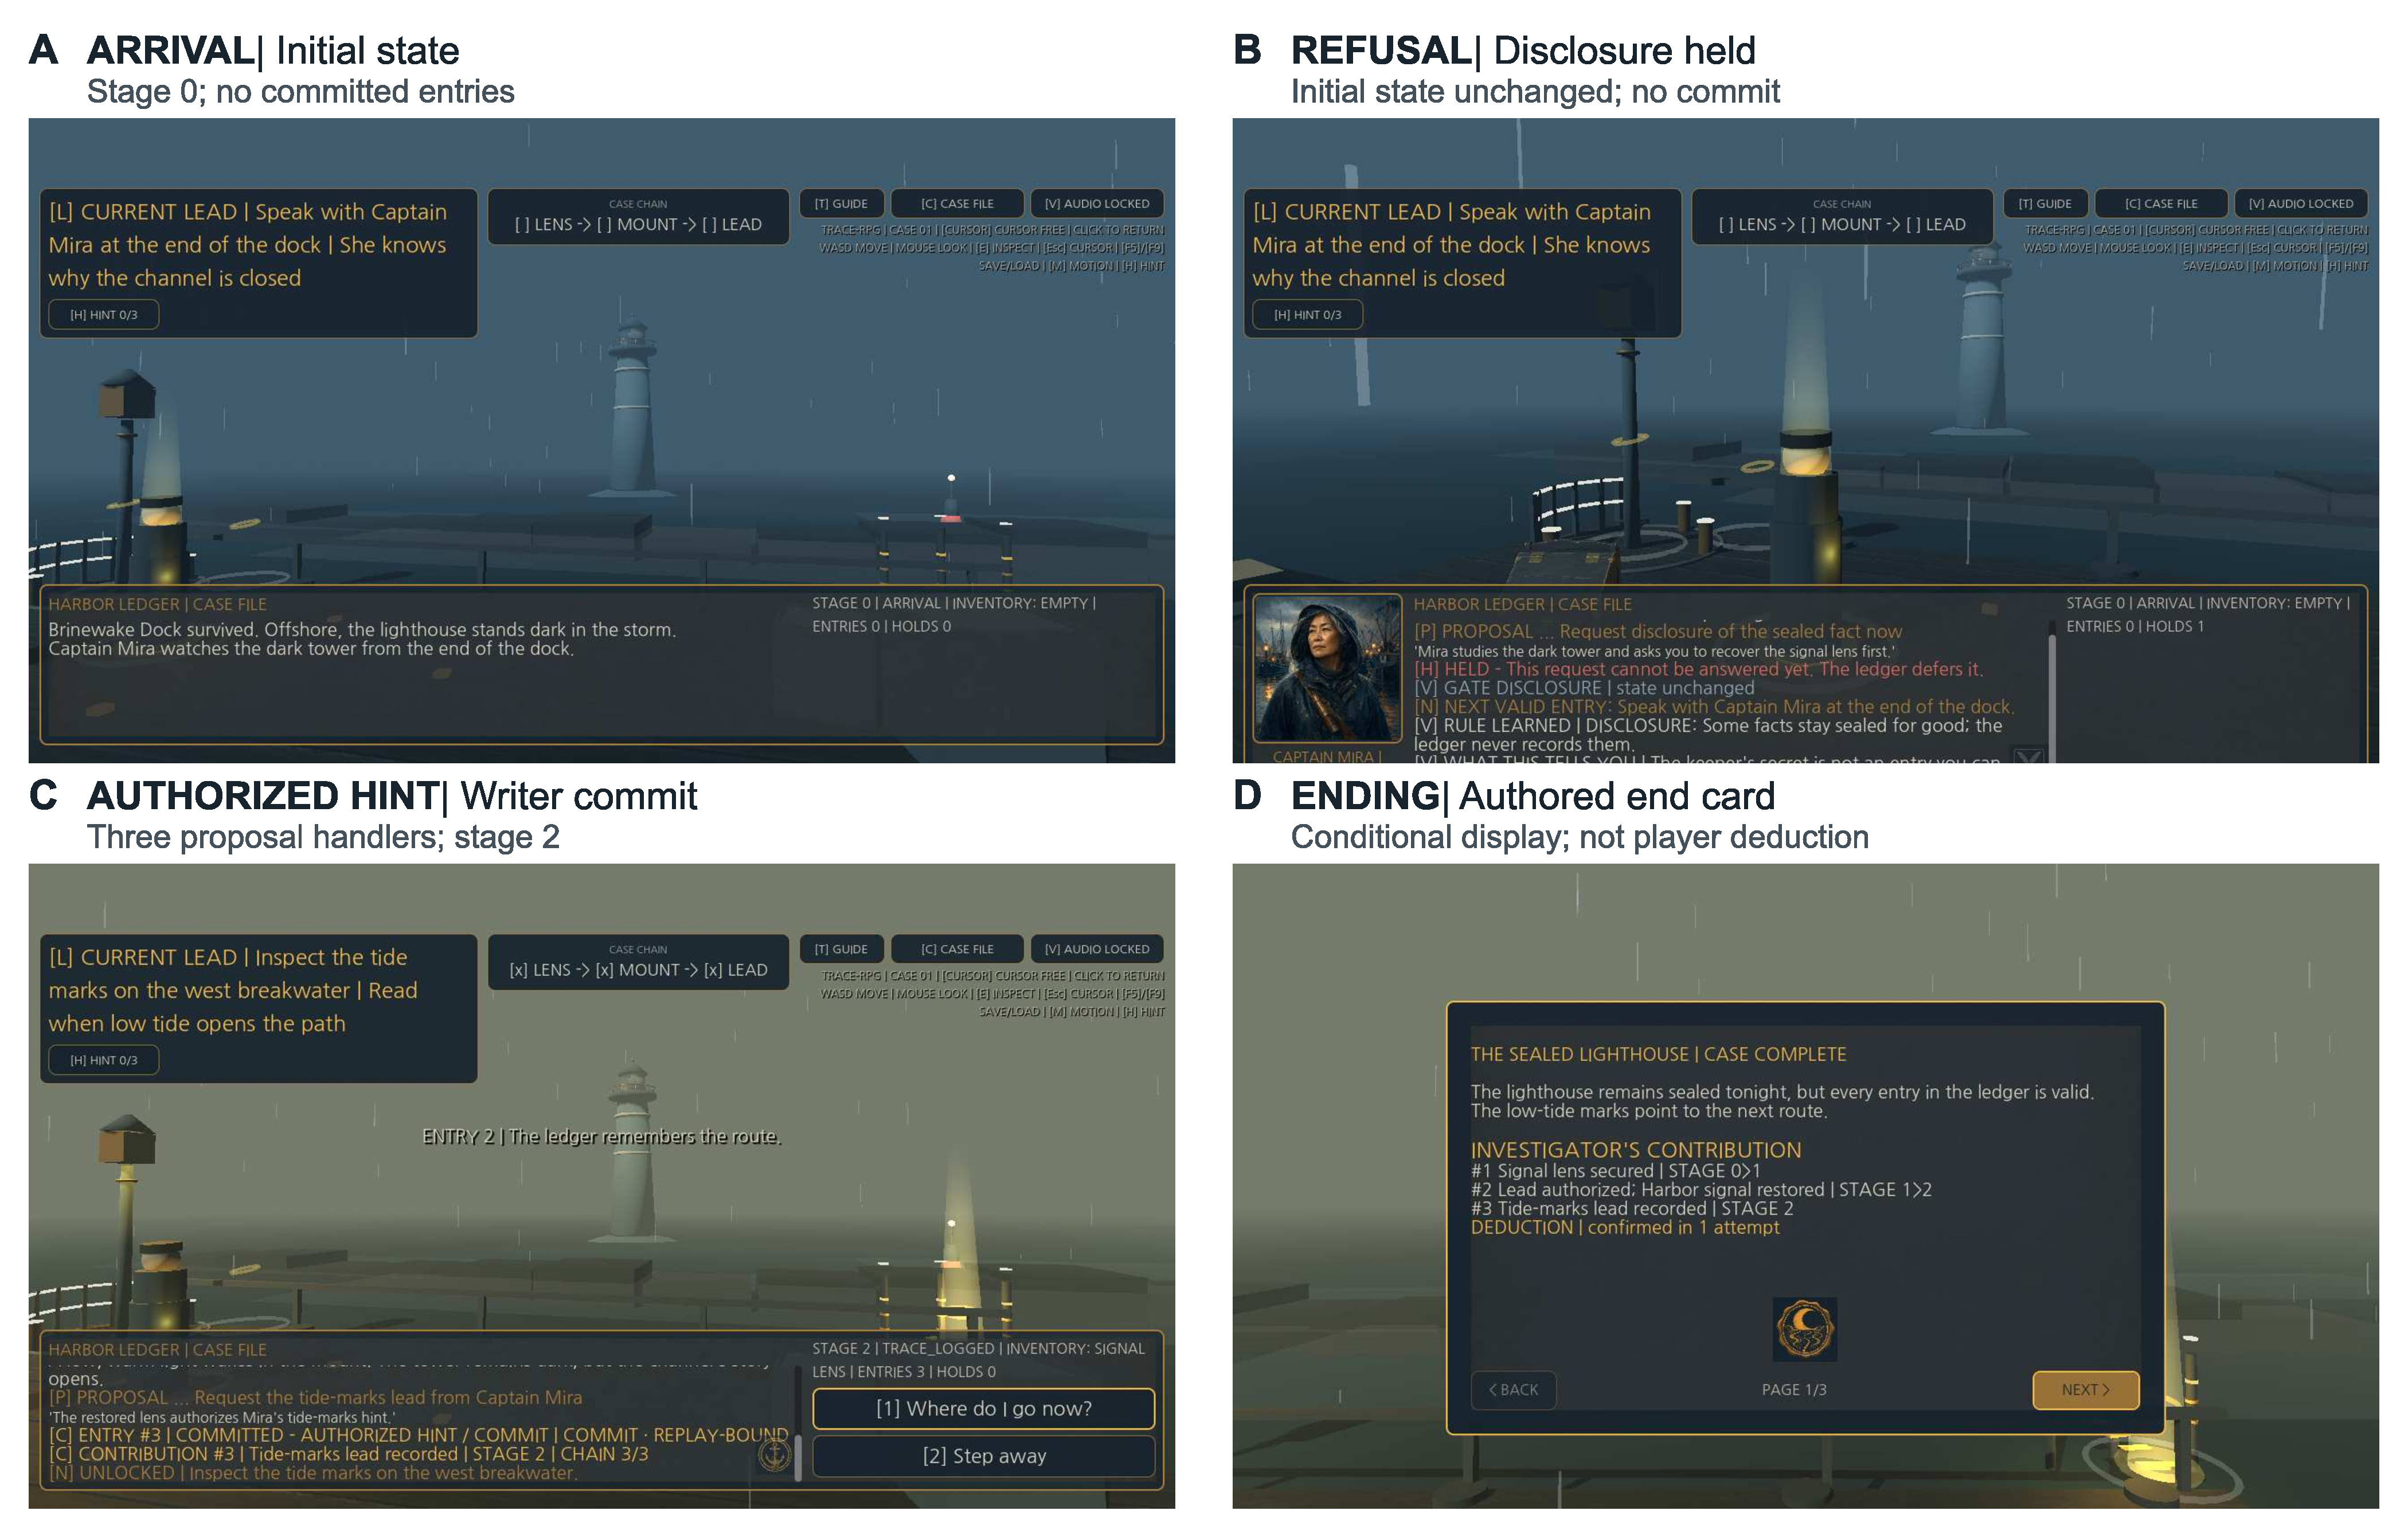
\includegraphics[width=0.90\textwidth]{../../figures/fig_engine_cutscenes.pdf}
\caption{Native Godot~4.7.1 engineering captures: (A)~initial arrival; (B)~denied premature secret disclosure with canonical state preserved; (C)~stage-2 authorized hint; (D)~conditional closing card.}
\Description{Four-panel Godot 4.7.1 screenshot sequence verifying engine state correspondence across arrival, denied disclosure, stage-2 hint, and closing card.}
\label{fig:engine-cutscenes}
\end{figure*}

\begin{figure}[!tbp]
\centering
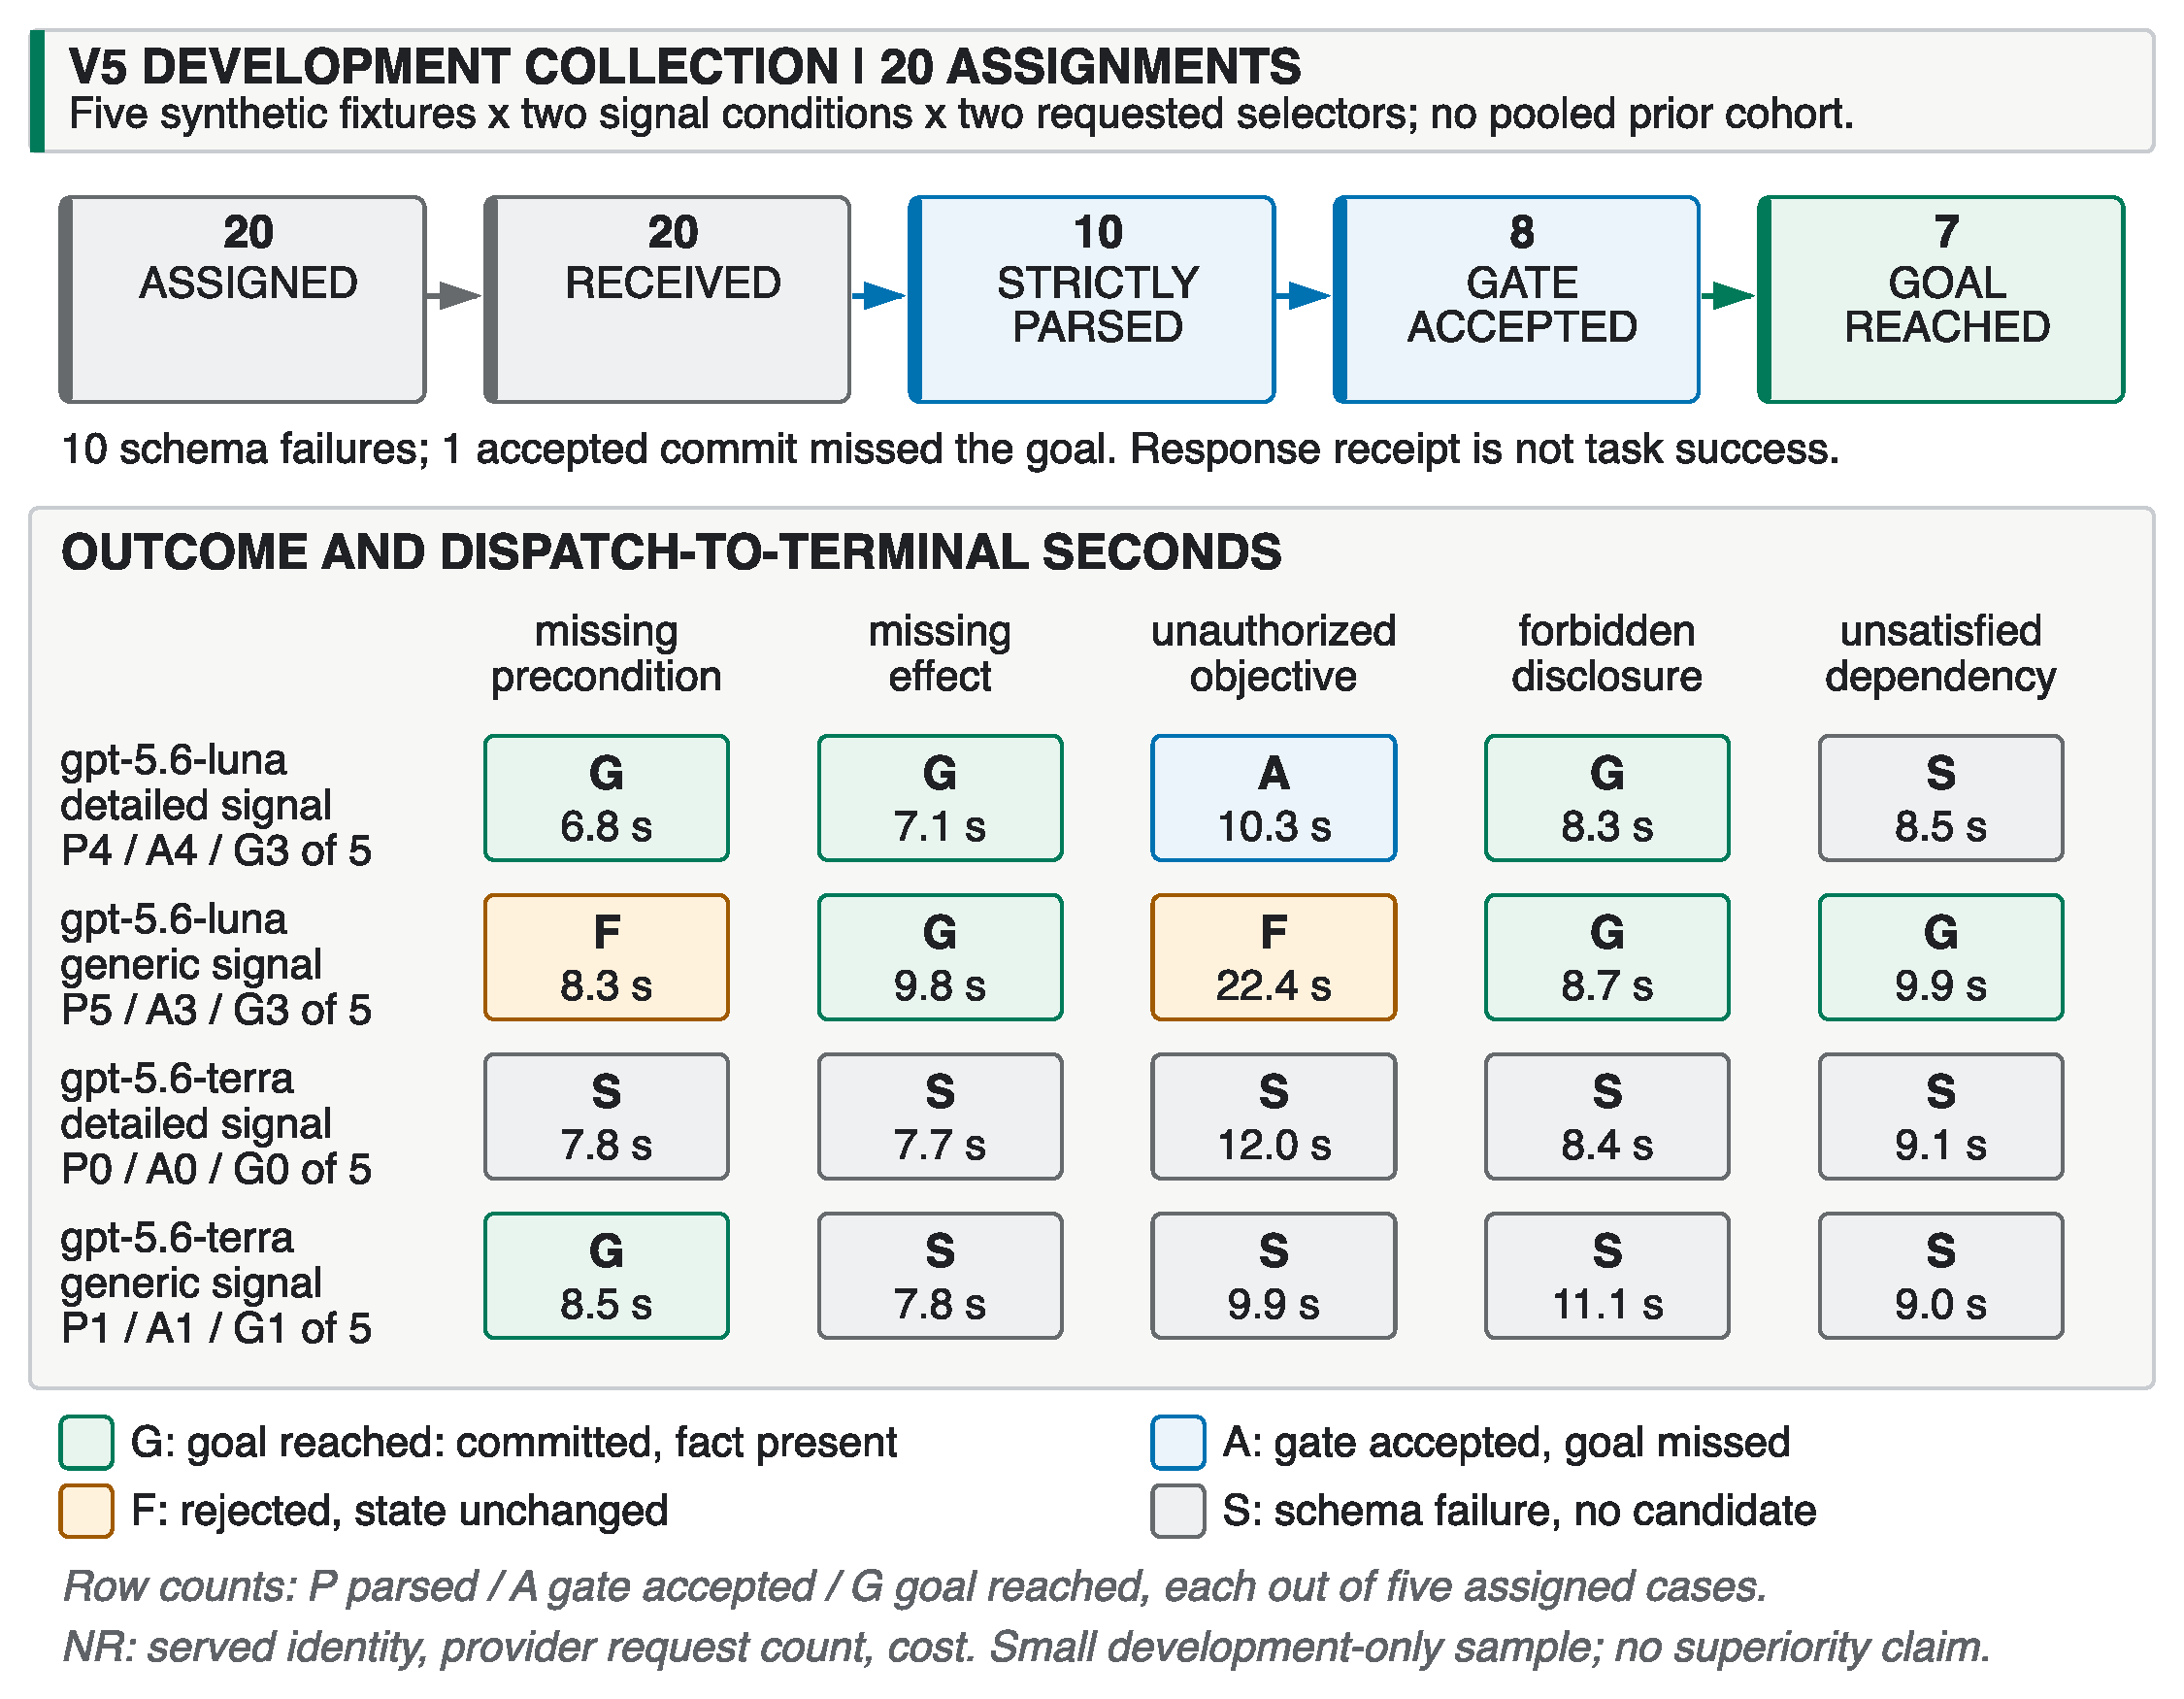
\includegraphics[width=\columnwidth]{../../figures/fig_paired_feedback_flow.pdf}
\caption{Assignment-complete flow on the 20-case synthetic collection: 10 schema failures remain in the denominator while 8 accepted candidates yield 7 goals.}
\Description{Sankey-style flow diagram across 20 assignments showing 10 parse failures, 8 gate passes, and 7 goal completions.}
\label{fig:paired-feedback-flow}
\end{figure}

\begin{table}[!tbp]
\caption{Zero-LLM Deterministic Boundary, Audit A1--A4, and Datalog Scaling (\textbf{P9}: 480 Procedural Cases)}
\label{tab:kbs-det}
\centering
\scriptsize
\setlength{\tabcolsep}{3pt}
\begin{tabularx}{\columnwidth}{@{}lcccc@{}}
\toprule
\textbf{Datalog Gate ($R{\le}64, d{\le}5$)} & \textbf{Acc.\ (480)} & \textbf{Leaks} & \textbf{Med.\ ($\mu$s)} & \textbf{p95 ($\mu$s)} \\
\midrule
\texttt{schema\_only} / \texttt{affordance} & 16.67\% (80) & 400 & --- & --- \\
\texttt{flat\_1hop\_gate} & 46.67\% (224) & 256 & 0.87--1.57 & 1.37--2.18 \\
\texttt{bounded\_2hop\_gate} & 60.00\% (288) & 192 & 1.88--2.58 & 2.66--3.91 \\
\texttt{nesy\_game.multihop} & \textbf{100.0\% (480)} & \textbf{0} & \textbf{6.46--7.12} & 9.83--11.42 \\
\bottomrule
\end{tabularx}
\end{table}

\subsection{Formal KR Translation Encodings: ASP, SMT-LIB, and OWL~2~RL}\label{sec:kr-encodings}
To demonstrate that \system{}'s runtime authorization semantics are solver-agnostic, we formally translate the ontology graph $\mathcal{G} = (\mathcal{V}, \mathcal{E}, \tau)$, dynamic state $\sigma$, and proposed action $a = (\mathit{actor}, \mathit{verb}, \mathit{target})$ into three canonical Knowledge Representation formalisms: Answer Set Programming (ASP) via Clingo~\cite{gebser2019clingo}, Satisfiability Modulo Theories (SMT-LIB v2) via Z3~\cite{demoura2008z3}, and Description Logics via W3C OWL~2~RL~\cite{motik2012owl2profiles}.

\paragraph{1. ASP (Clingo) Encoding}
The ontology graph and game state map to ground relational facts $\texttt{edge}(u, v, r)$, $\texttt{entity\_at}(e, u)$, $\texttt{unlocked}(u, v)$, and $\texttt{secret\_stage}(e, s)$. Transitive topological accessibility and authorization constraints are declared through stratified Datalog with default negation:
{\footnotesize
\begin{align}
\texttt{passable}(U, V) &\leftarrow \texttt{edge}(U, V, \texttt{leadsTo}),\, \texttt{unlocked}(U, V). \label{eq:asp-passable} \\
\texttt{reachable}(U, V) &\leftarrow \texttt{passable}(U, V). \label{eq:asp-base} \\
\texttt{reachable}(U, W) &\leftarrow \texttt{reachable}(U, V),\, \texttt{passable}(V, W). \label{eq:asp-trans} \\
\texttt{accessible}(E) &\leftarrow \texttt{player\_at}(L_0),\, \texttt{entity\_at}(E, L_0). \label{eq:asp-local} \\
\texttt{accessible}(E) &\leftarrow \texttt{player\_at}(L_0),\, \texttt{reachable}(L_0, L),\notag\\
&\quad \texttt{entity\_at}(E, L). \label{eq:asp-remote} \\
\texttt{authorized}(a) &\leftarrow \texttt{prop}(a, \mathit{Act}, \mathit{Tgt}),\, \texttt{accessible}(\mathit{Tgt}),\notag\\
&\quad \textbf{not } \texttt{leak}(a). \label{eq:asp-auth} \\
\texttt{leak}(a) &\leftarrow \texttt{prop}(a, \mathit{Act}, \mathit{Tgt}),\, \texttt{secret}(\mathit{Tgt}),\notag\\
&\quad \textbf{not } \texttt{stage\_cleared}(\mathit{Tgt}). \label{eq:asp-leak} \\
&\leftarrow \texttt{prop}(a, \cdot, \cdot),\, \textbf{not } \texttt{authorized}(a). \label{eq:asp-integrity}
\end{align}}
Grounding through \texttt{gringo} and solving through \texttt{clasp}~\cite{gebser2019clingo} produces exactly one stable model iff $a$ is admissible.

\paragraph{2. SMT-LIB / Z3 Encoding}
In first-order SMT-LIB v2 with uninterpreted sorts $\text{Loc}$ and $\text{Ent}$, transitive reachability is axiomatized over binary relations $\texttt{passable}: \text{Loc} \times \text{Loc} \to \text{Bool}$ and $\texttt{reach}: \text{Loc} \times \text{Loc} \to \text{Bool}$, bounded by inductive distance $\texttt{dist}: \text{Loc} \times \text{Loc} \to \text{Int}$:
\begin{align}
\forall u, v.\; &\texttt{passable}(u, v) \implies \texttt{reach}(u, v) \land (\texttt{dist}(u, v) = 1), \label{eq:smt-base} \\
\forall u, v, w.\; &\bigl(\texttt{reach}(u, v) \land \texttt{passable}(v, w)\bigr) \implies \notag \\
&\quad \bigl(\texttt{reach}(u, w) \land (\texttt{dist}(u, w) \le \texttt{dist}(u, v) + 1)\bigr). \label{eq:smt-trans}
\end{align}
Admissibility is posed as satisfiability of the conjunction $\Phi_{\mathrm{axioms}} \land \Phi_{\mathrm{state}} \land \Phi_{\mathrm{auth}}(a)$. Checking consistency via Z3~\cite{demoura2008z3} evaluates proposal validity through model existence.

\paragraph{3. OWL~2~RL Translation}
Under the W3C OWL~2~RL profile~\cite{motik2012owl2profiles}, relational reachability is modeled as an OWL object property hierarchy. Transitivity is asserted via $\texttt{SubObjectPropertyOf}(\texttt{ObjectPropertyChain}(:\texttt{passable} \; :\texttt{passable}) \; :\texttt{reachable})$ alongside $\texttt{TransitiveObjectProperty}(:\texttt{reachable})$. Entities are mapped to OWL named individuals, and state authorization checks correspond to forward-chaining Rete materialization over an in-memory RDF graph using RDFLib~7.6.0 and OWLRL~7.6.2.

\paragraph{Semantic Equivalence Theorem}
\textit{For any finite game ontology $\mathcal{G}$, consistent state $\sigma$, and proposed action $a$, the dedicated engine $\Valid(a, \sigma)$ evaluates to true if and only if $\mathcal{T}_{\mathrm{ASP}}(\mathcal{G}, \sigma, a)$ has an answer set, $\mathcal{T}_{\mathrm{SMT}}(\mathcal{G}, \sigma, a)$ is SAT, and $\mathcal{T}_{\mathrm{OWL}}(\mathcal{G}, \sigma, a) \models \texttt{AuthorizedAction}(a)$.}

\subsection{Cross-Solver Benchmarks and Asymptotic Frame-Budget Cliffs (\textbf{P18A} \& \textbf{P18B})}\label{sec:kr-benchmarks}
We benchmark all four KR engines on Python~3.11.14 (\texttt{nesy\_game} 0.1.0, Clingo 5.8.3, Z3 5.4.1.0, RDFLib 7.6.0 + OWLRL 7.6.2). In \textbf{P18A} (Table~\ref{tab:p18a}), all 120 five-world test instances (24 cases/world $\times$ 5 worlds) yield \textbf{0/120 mismatches} across all four engines, empirically validating semantic equivalence. However, latency diverges by four orders of magnitude: \texttt{nesy\_game} requires median 2.46\,$\mu$s (p95 3.60\,$\mu$s), Clingo requires 397.12\,$\mu$s, Z3 requires 2.634\,ms, and OWL~2~RL requires 19.223\,ms. While \texttt{nesy\_game}, Clingo, and Z3 achieve 100\% compliance with 60\,Hz (16.67\,ms) and 120\,Hz (8.33\,ms) interactive frame budgets, OWL~2~RL fails 60\,Hz deadlines on 100\% of instances.

\begin{table}[!tbp]
\caption{Cross-Engine Semantic Equivalence and Frame Compliance (\textbf{P18A}: 5 Worlds $\times$ 24 Cases = 120 Cases)}
\label{tab:p18a}
\centering
\scriptsize
\setlength{\tabcolsep}{2.5pt}
\begin{tabularx}{\columnwidth}{@{}>{\raggedright\arraybackslash}Xcccc@{}}
\toprule
\textbf{KR Engine / Solver} & \textbf{Acc.\ (120)} & \textbf{Med.\ ($\mu$s)} & \textbf{p95 ($\mu$s)} & \textbf{60/120\,Hz Pass} \\
\midrule
\texttt{nesy\_game} 0.1.0 & \textbf{120/120 (100\%)} & \textbf{2.46} & \textbf{3.60} & \textbf{100\% / 100\%} \\
Clingo 5.8.3 (ASP)~\cite{gebser2019clingo} & \textbf{120/120 (100\%)} & 397.12 & 507.90 & \textbf{100\% / 100\%} \\
Z3 5.4.1.0 (SMT-LIB)~\cite{demoura2008z3} & \textbf{120/120 (100\%)} & 2,634.0 & 3,338.0 & \textbf{100\% / 100\%} \\
OWL~2~RL (RDFLib/OWLRL)~\cite{motik2012owl2profiles} & \textbf{120/120 (100\%)} & 19,223.0 & 20,362.0 & 0\% / 0\% \\
\bottomrule
\end{tabularx}
\end{table}

\begin{table*}[!tbp]
\caption{Procedural Graph Scaling, External KR Solvers, and Asymptotic Frame-Budget Cliffs (\textbf{P18B}: 1,080 Instances Across 3 Topologies)}
\label{tab:p18b}
\centering
\scriptsize
\setlength{\tabcolsep}{2.5pt}
\begin{tabularx}{\textwidth}{@{}>{\raggedright\arraybackslash}Xcccccccccc@{}}
\toprule
\textbf{KR Solver / Baseline} & \textbf{Acc.\ (1080)} & \textbf{Med.\ (ms)} & \textbf{p95 (ms)} & \textbf{60\,Hz Pass} & \textbf{$R{=}8$} & \textbf{$R{=}16$} & \textbf{$R{=}32$} & \textbf{$R{=}64$} & \textbf{$R{=}128$} & \textbf{$R{=}256$} \\
\midrule
\texttt{nesy\_game.multihop} & \textbf{1080/1080 (100\%)} [99.7, 100] & \textbf{0.032} & \textbf{0.362} & \textbf{100.0\%} & \textbf{0.019} & \textbf{0.029} & \textbf{0.050} & \textbf{0.093} & \textbf{0.179} & \textbf{0.354} \\
\texttt{clingo\_asp} (5.8.3)~\cite{gebser2019clingo} & \textbf{1080/1080 (100\%)} [99.7, 100] & 1.268 & 6.600 & \textbf{100.0\%} & 0.452 & 0.639 & 1.002 & 1.679 & 3.017 & 5.721 \\
\texttt{z3\_smt} (5.4.1.0)~\cite{demoura2008z3} & \textbf{1080/1080 (100\%)} [99.7, 100] & 7.885 & 41.084 & 68.43\% & 1.840 & 2.964 & 5.257 & 9.443 & \textit{17.447} & \textbf{34.670} \\
\texttt{owl2\_rl} (RDFLib/OWLRL)~\cite{motik2012owl2profiles} & 45/45* (100\%) [92.1, 100] & 486.39 & --- & 0.0\% & 114.50 & 486.39 & 2,796.11 & 19,696.18 & $>$20\,s & $>$20\,s \\
\texttt{flat\_1hop\_gate} & 540/1080 (50.00\%) [47.0, 53.0] & 0.0008 & 0.0012 & 100.0\% & 0.0007 & 0.0008 & 0.0008 & 0.0008 & 0.0009 & 0.0009 \\
\texttt{bounded\_2hop\_gate} & 630/1080 (58.33\%) [55.4, 61.2] & 0.0020 & 0.0031 & 100.0\% & 0.0018 & 0.0019 & 0.0020 & 0.0021 & 0.0022 & 0.0023 \\
\bottomrule
\end{tabularx}
\vspace{1ex}
\raggedright\scriptsize\textit{Note:} Per-scale columns report median latency in ms. Z3 60\,Hz frame-budget compliance drops sharply at $R{\ge}128$ (100\% at $R{\le}32$, 98.89\% at $R{=}64$, 11.67\% at $R{=}128$, 0.0\% at $R{=}256$). *OWL~2~RL evaluated on 45 stratified cases (165/165 total including P18A without mismatch); instances at $R{\ge}128$ exceed the 20\,s execution safety cutoff due to cubic materialization complexity.
\end{table*}

To characterize scalability, \textbf{P18B} evaluates 1,080 procedurally generated graph instances crossing six room counts ($R \in \{8, 16, 32, 64, 128, 256\}$), six query path depths ($d \in \{1, 2, 3, 5, 8, 10\}$), three topologies (linear chain, balanced branching tree, and diamond mesh), and 10 random seeds per cell (Table~\ref{tab:p18b}). Cochran's test confirms massive performance disparity across the five complete evaluators ($Q = 1948.24, \text{df}=4, p < 10^{-300}$). Pairwise exact McNemar tests confirm that while \texttt{clingo\_asp} and \texttt{z3\_smt} achieve identical semantic accuracy to \texttt{nesy\_game} ($p = 1.000$, zero discordant pairs), \texttt{flat\_1hop} (50.00\%) and \texttt{bounded\_2hop} (58.33\%) collapse on multi-hop paths ($p < 10^{-100}$).

Crucially, \textbf{P18B} reveals two distinct asymptotic \textit{frame-budget cliffs}:
\begin{enumerate}
\item \textbf{Z3 SMT Quantifier Cliff ($R \ge 128$):} In general first-order SMT-LIB solvers, transitive reachability requires universal quantifiers. While E-matching heuristic instantiation solves small instances quickly ($1.84$\,ms at $R{=}8$, $5.26$\,ms at $R{=}32$), ground clause generation escalates steeply. At $R{=}128$, median latency hits $17.447$\,ms, breaching the 60\,Hz deadline (16.67\,ms) and collapsing 60\,Hz frame pass rate from 98.89\% ($R{=}64$) to \textbf{11.67\%}. At $R{=}256$, median latency reaches $34.670$\,ms (p95 $41.08$\,ms), resulting in \textbf{0.0\%} 60\,Hz frame compliance.
\item \textbf{OWL~2~RL Cubic Materialization Cliff ($R \ge 128$):} Forward-chaining rule materialization in OWL~2~RL exhibits worst-case $O(n^3)$ cubic time complexity in the number of individuals for transitive property composition. In RDFLib/OWLRL, median latency climbs from $114.50$\,ms ($R{=}8$) to $486.39$\,ms ($R{=}16$), $2,796.11$\,ms ($R{=}32$), and $19,696.18$\,ms ($R{=}64$). At $R \ge 128$, reasoning exceeds the 20-second safety cutoff ($>20$\,s/case), making standard OWL~2~RL engines unusable for interactive game runtimes.
\end{enumerate}
In contrast, \texttt{nesy\_game.multihop} implements dedicated in-memory bitset adjacency closure operating in $O(|\mathcal{V}| + |\mathcal{E}|)$. It scales smoothly from $0.019$\,ms ($R{=}8$) to $0.354$\,ms ($R{=}256$, p95 $0.456$\,ms), sustaining \textbf{100.0\%} compliance across both 60\,Hz and 120\,Hz budgets. Clingo ASP also sustains 100\% 60/120\,Hz compliance ($0.452$\,ms at $R{=}8$ to $5.721$\,ms at $R{=}256$), but is $\approx$40$\times$ slower than \texttt{nesy\_game} due to grounding process overhead.

\subsection{Independent Closed-Loop 7-Arm Shielding and Cross-Family Negotiation (\textbf{P15} \& \textbf{P11})}\label{sec:kbs-mas}
Table~\ref{tab:kbs-mas} reports \textbf{P15} (\textbf{105 independent 5-turn closed-loop trajectories} across Haiku, Sonnet, Opus~5.5 $\times$ 5 worlds $\times$ 7 arms; 1,048,803 tokens; \textbf{105/105} fresh 0-LLM replays exact) together with model-tier breakdowns. Controlled Safe-RL proxy masking~\cite{alshiekh2018shield} (0/15 safe goals, 1/15 zero-leak, 16/61 unsafe turns) and NeMo-style Colang proxy rails~\cite{rebedea2023nemo} (1/15, 1/15, 15/61) miss multi-hop derived and knowledge violations, and flat 1-hop gating still leaks 4/66 turns across 3/15 episodes in complex worlds (\texttt{ivory-citadel-v1}: 2 unsafe turns in 1/3 episode; \texttt{glass-foundry-v1}: 2 unsafe turns in 2/3 episodes). All three \texttt{nesy\_game.multihop} arms sustain \textbf{15/15 (100.0\% [79.61\%, 100.0\%])} zero-leak protection and \textbf{0} unsafe commits across all 3 tiers and all 5 worlds (3/3 per world). Crucially, every rejected candidate across \texttt{multihop\_k0} and \texttt{trace\_rpg\_multihop\_rho\_k2} in \textbf{P15} is a Theorem-2 state-dependent epistemic/stage violation, so $\rho$ maps all 18 blocked calls in \texttt{rho\_k2} to identity (\texttt{rho\_repairs=0}; the 14/15 [93.33\%] vs.\ 13/15 [86.67\%] difference over \texttt{k0} stems from independent Turn-1 LLM sampling on \texttt{haiku::ivory-citadel-v1}, not $\rho$ edits), whereas hybrid $\rho{+}\text{LLM}_{K=1}$ clears dead-ends via 20 Theorem-2 safe re-targets to reach \textbf{15/15 (100.0\%)} across Haiku, Sonnet, and Opus ($Q_{\mathrm{goal}}{=}68.714, p{=}7.50{\times}10^{-13}$; $Q_{\mathrm{zl}}{=}71.651, p{=}1.87{\times}10^{-13}$; McNemar vs.\ Safe-RL/NeMo $p{\le}1.22{\times}10^{-4}$). External 3-family CLI negotiation (\textbf{P11}: 30 episodes crossing Claude~Sonnet~5.5, open-weight GPT-OSS~120B, and Gemini~4~Hydrogen, 79/90 parsed, 11 GPT-OSS PF kept) confirms \textbf{30/30} zero-leak, 16/30 milestones, and \textbf{0/79} unsafe turns vs.\ Safe-RL (37/79, $p{=}9.5{\times}10^{-7}$), NeMo (43/79, $p{=}1.2{\times}10^{-7}$), and flat (29/79, $Q{=}118.93$).

\begin{table*}[!tbp]
\caption{Independent Closed-Loop 7-Arm Shielding with Exact Repair and Per-Tier Breakdown (\textbf{P15}: 105 Attested Episodes, 105/105 0-LLM Replays Valid)}
\label{tab:kbs-mas}
\centering
\scriptsize
\setlength{\tabcolsep}{3.0pt}
\begin{tabularx}{\textwidth}{@{}>{\raggedright\arraybackslash}Xcccccccc@{}}
\toprule
\textbf{Shielding Arm (15 ep/arm)} & \textbf{Safe Goal (95\% CI)} & \textbf{Zero-Leak} & \textbf{Unsafe} & \textbf{Blk/$\rho$/PF/Ret} & \textbf{Haiku} & \textbf{Sonnet} & \textbf{Opus} & \textbf{Tokens} \\
\midrule
\texttt{schema\_only} & 2/15 (13.3\%) [3.7, 37.9] & 2/15 & 16/59 & 0 / 0 / 0 / 0 & 1/1/6 & 1/1/4 & 0/0/6 & 133,054 \\
\texttt{safe\_rl\_action\_mask}~\cite{alshiekh2018shield} & 0/15 (0.0\%) [0.0, 20.4] & 1/15 & 16/61 & 2 / 0 / 0 / 0 & 0/1/5 & 0/0/5 & 0/0/6 & 139,205 \\
\texttt{nemo\_colang\_rail}~\cite{rebedea2023nemo} & 1/15 (6.7\%) [1.2, 29.8] & 1/15 & 15/61 & 1 / 0 / 1 / 0 & 0/0/5 & 0/0/5 & 1/1/5 & 136,515 \\
\texttt{flat\_1hop\_shield} & 12/15 (80.0\%) [54.8, 93.0] & 12/15 & 4/66 & 15 / 0 / 0 / 0 & 4/4/1 & 5/5/0 & 3/3/3 & 146,446 \\
\texttt{multihop\_shield\_k0} & 13/15 (86.7\%) [62.1, 96.3] & \textbf{15/15} & \textbf{0/69} & 22 / 0 / 0 / 0 & 4/5/0 & 5/5/0 & 4/5/0 & 152,649 \\
\texttt{trace\_rpg\_multihop\_rho\_k2} & 14/15 (93.3\%) [70.2, 98.8] & \textbf{15/15} & \textbf{0/68} & 18 / 0 / 0 / 0 & 5/5/0 & 5/5/0 & 4/5/0 & 150,986 \\
\texttt{trace\_rpg\_hybrid\_rho\_llm\_k1} & \textbf{15/15 (100\%)} [79.6, 100] & \textbf{15/15} & \textbf{0/63} & 2 / 0 / 1 / 20 & \textbf{5/5/0} & \textbf{5/5/0} & \textbf{5/5/0} & 189,948 \\
\bottomrule
\end{tabularx}
\end{table*}

\subsection{Attested Prospective Factorial Ablations (\textbf{P16A}) and Fair $(a,E)$ Repair (\textbf{P12})}\label{sec:kbs-p16a}
Table~\ref{tab:kbs-p16a} disaggregates all 60 prospective factorial episodes of \textbf{P16A} across representation, model tier, and quest world (673,869 tokens, non-pooled with frozen 0/180 \texttt{20261103}). Under \texttt{general\_rule}, Sonnet (4 unsafe commits) and Opus (5 unsafe commits) breach multi-hop knowledge/role checks in \texttt{ivory-citadel-v1} (4) and \texttt{glass-foundry-v1} (5), yielding 0/30 goals and 22/30 (73.33\%) zero-leak. Switching to \texttt{ontology\_multihop} enforces \textbf{30/30 (100.0\%)} zero-leak (McNemar $p{=}0.00781$), \textbf{0} unsafe commits across every tier and world, 22 runtime repairs (Haiku 18, Sonnet 4), and \textbf{11/30 (36.67\%)} safe goals (Opus 8/10, Sonnet 3/10, Haiku 0/10; $p{=}9.77{\times}10^{-4}$). Complementing this factorial test, \textbf{P12} (90 5-world proposals, 84/90 parsed) confirms \textbf{0/84} unsafe commits only under \system{} vs.\ Safe-RL (54/84), NeMo (55/84), and flat 1-hop (32/84; $Q{=}281.23$); on 27 matched policy+stage faults given equal $(a,E)$ counterexamples, deterministic $\rho_{K=2}$ hits \textbf{27/27 (100.0\%)} at 0 extra tokens vs.\ matched State-Blind and State-Aware LLM $K{=}2$ (both 26/27 = 96.3\% at 530,044--542,042 extra tokens / $>$508\,s, $p{=}1.0$), isolating zero-token latency elimination and Theorem~2 non-laundering fallback.

\begin{table}[!tbp]
\caption{Per-Tier and Per-World Disaggregation in Attested Factorial Suite (\textbf{P16A}: 60 Episodes; \texttt{gen}/\texttt{ont} = \texttt{general\_rule}/\texttt{ontology\_multihop})}
\label{tab:kbs-p16a}
\centering
\scriptsize
\setlength{\tabcolsep}{1.5pt}
\begin{tabularx}{\columnwidth}{@{}>{\raggedright\arraybackslash}X*{6}{c}@{}}
\toprule
\textbf{Stratum} & \textbf{Goal (\texttt{g/o})} & \textbf{Zero-Leak} & \textbf{Unsf.} & \textbf{Rep.} & \textbf{PF} & \textbf{Tok (k)} \\
\midrule
Overall (30/30) & 0/30 / \textbf{11/30} & 22/30 / \textbf{30/30} & 9/\textbf{0} & 0/22 & 1/1 & 294/380 \\
\texttt{claude-haiku} & 0/10 / 0/10 & 10/10 / 10/10 & 0/0 & 0/18 & 0/1 & 104/138 \\
\texttt{claude-sonnet} & 0/10 / 3/10 & 6/10 / \textbf{10/10} & 4/\textbf{0} & 0/4 & 0/0 & 104/130 \\
\texttt{claude-opus} & 0/10 / \textbf{8/10} & 6/10 / \textbf{10/10} & 5/\textbf{0} & 0/0 & 1/0 & 85/112 \\
\midrule
\texttt{lighthouse} & 0/6 / 2/6 & 6/6 / 6/6 & 0/0 & 0/6 & 0/1 & 59/75 \\
\texttt{archive} & 0/6 / 0/6 & 6/6 / 6/6 & 0/0 & 0/8 & 0/0 & 60/79 \\
\texttt{observatory} & 0/6 / 2/6 & 6/6 / 6/6 & 0/0 & 0/2 & 0/0 & 61/77 \\
\texttt{ivory-citadel} & 0/6 / 3/6 & 2/6 / \textbf{6/6} & 4/\textbf{0} & 0/4 & 1/0 & 58/79 \\
\texttt{glass-foundry} & 0/6 / \textbf{4/6} & 2/6 / \textbf{6/6} & 5/\textbf{0} & 0/2 & 0/0 & 55/70 \\
\bottomrule
\end{tabularx}
\end{table}

\subsection{Authentic Headless Godot~4.7.1 Multi-World and 5,000-Tick Soak Execution (\textbf{P16B}, \textbf{P13}, \& \textbf{P19})}\label{sec:kbs-godot}
In attested live Godot~4.7.1 execution (\textbf{P16B}: 21 closed-loop episodes across Haiku, Sonnet, Opus~5.5, 169,071 tokens), every trajectory re-executes inside headless Godot~4.7.1 (\texttt{4.7.1.\allowbreak stable.\allowbreak official.\allowbreak a13da4feb}) with 0 LLM calls at verification time: \textbf{21/21} fresh replays pass, \textbf{0/21} unsafe commits/leaks occur, \textbf{13/15} five-world goals succeed (Haiku 5/5, Sonnet 4/5, Opus 4/5; Godot runtime 251.64--1009.78\,ms vs.\ API 10,606--40,892\,ms), and \textbf{6/6 (100.0\%)} production \texttt{SealedLighthouseMachine} runs under both \texttt{standard} and \texttt{social\_pressure} regimes match \texttt{EXACT\_\allowbreak TERMINAL\_\allowbreak HASH} (\texttt{4b231017...}; Godot 751.30--778.80\,ms vs.\ API 9,055--16,485\,ms). This parallels 3-family CLI Godot~4.7.1 results (\textbf{P13}: 42/42 replays valid, 0/42 leaks, Claude \& Hydrogen 14/14 goals vs.\ GPT-OSS 4/14).

Extending this to long-horizon engine soak, \textbf{P19} executes two authentic Godot~4.7.1 verification batteries:
\begin{enumerate}
\item \textbf{Five-World Deterministic Parity (120 Cases):} Headless Godot runs 24 procedural instances across all five quest worlds. GDScript execution reaches \textbf{120/120 (100.0\%)} bit-level parity against the Python reference kernel (0 divergences) at median latency 5.0\,$\mu$s (p95 8.0\,$\mu$s). Across all 5/5 quest worlds, full episodic trajectories match fresh-process SHA-256 state hashes identically.
\item \textbf{5,000-Tick Multi-Tier Soak:} To evaluate memory stability and frame budget limits under prolonged gameplay, Godot runs a 5,000-tick soak across five scaling tiers ($R \in \{8..128\}$, action space $A \in \{3..16\}$, path depth $d \in \{2..8\}$). Across all 5,000 ticks, the engine processes 3,750 valid action commits, executes 1,250 state-blind $\rho$-repairs, and intercepts \textbf{1,875 blocked leaks} with \textbf{0 unsafe commits} and \textbf{0 state leaks}. Peak single-tick latency is 0.074\,ms (74\,$\mu$s), comfortably preserving \textbf{100\%} compliance with 60\,Hz and 120\,Hz render budgets.
\end{enumerate}

\subsection{Unified Stage-1 + Stage-2 Bilingual Escape and 1,200-Case LODO Benchmark (\textbf{P17}, \textbf{P14}, \& \textbf{P20})}\label{sec:kbs-escape}
Table~\ref{tab:kbs-p17} details \textbf{P17}: \textbf{540} fresh API evaluations using one identical prompt across 180 EN/KO cases (90 EN, 90 KO; 3 domains $\times$ 60 cases; 0 deterministic short-circuits, 359,030 tokens; Fleiss' $\kappa{=}0.8813$, $\alpha{=}0.8815$, $Q{=}9.5, p{=}0.00865$). Every Claude~5.5 tier achieves \textbf{0/72 (0.0\%) FRR} and 94.44--97.22\% paraphrase recall (significantly outperforming calibrated rule hybrid on Haiku $p{=}1.12{\times}10^{-4}$ and Opus $p{=}0.00940$, with no language collapse across EN/KO). Yet neural tiers miss 7--17/36 unhinted explicit ID tokens inside neutral prose (especially \texttt{keeper\_secret}: Sonnet 2/12, Haiku/Opus 5/12), demonstrating why symbolic Stage-1 gating (36/36 explicit) and Stage-2 neural detection must operate jointly. Cross-family 720-eval checks (\textbf{P14}) corroborate open-weight parity (\texttt{gpt-oss-120b-medium} $F_1{=}0.9714$, $\kappa{=}0.9367$).

\begin{table}[!tbp]
\caption{Unified-Prompt Bilingual Escape Disaggregation (\textbf{P17}: 180 EN/KO Cases $\times$ 3 Tiers = 540 Evals, 0 Short-Circuits)}
\label{tab:kbs-p17}
\centering
\scriptsize
\setlength{\tabcolsep}{1.4pt}
\begin{tabularx}{\columnwidth}{@{}>{\raggedright\arraybackslash}X*{6}{c}@{}}
\toprule
\textbf{Verifier} & \textbf{Exp} & \textbf{Para} & \textbf{FRR} & \textbf{$F_1$} & \textbf{EN/KO} & \textbf{Domains} \\
\midrule
\texttt{id\_only} & \textbf{36/36} & 0/72 & 0/72 & .500 & --- & .50/.50/.50 \\
\texttt{loo\_tfidf} & \textbf{36/36} & 45/72 & 45/72 & .692 & --- & .70/.66/.72 \\
\texttt{rule\_hybrid} & \textbf{36/36} & 38/72 & 0/72 & .813 & --- & .64/.94/.82 \\
\texttt{haiku-5-5} & 29/36 & \textbf{70/72} & \textbf{0/72} & \textbf{.957} & .95/.96 & .88/.99/\textbf{1.0} \\
\texttt{sonnet-5-5} & 19/36 & \textbf{70/72} & \textbf{0/72} & .904 & .92/.89 & .84/.89/.97 \\
\texttt{opus-5-5} & 25/36 & 68/72 & \textbf{0/72} & .925 & .94/.91 & .89/.89/.99 \\
\bottomrule
\end{tabularx}
\end{table}

\begin{table}[!tbp]
\caption{1,200-Case Bilingual Escape Benchmark Across 6 Domains (\textbf{P20}: LODO Generalization)}
\label{tab:p20}
\centering
\scriptsize
\setlength{\tabcolsep}{2.0pt}
\begin{tabularx}{\columnwidth}{@{}>{\raggedright\arraybackslash}Xcccc@{}}
\toprule
\textbf{Verifier / Method} & \textbf{Acc.\ (1200)} & \textbf{FRR} & \textbf{S4 FRR} & \textbf{Design} \\
\midrule
\texttt{stage1\_id\_only} & 60.00\% (720) & \textbf{0.00\%} & \textbf{0.00\%} & Symbolic Token \\
\texttt{keyword\_rule\_naive} & 62.67\% (752) & 75.21\% & 98.33\% & Naive Lexical \\
\texttt{stage1+neg\_hybrid} & 73.67\% (884) & \textbf{0.00\%} & \textbf{0.00\%} & Negation Regex \\
\texttt{bm25\_lexical\_lodo} & 96.75\% (1161) & 3.12\% & 2.08\% & Lexical LODO \\
\texttt{tfidf\_char\_word\_lodo} & \textbf{97.17\% (1166)} & 4.79\% & 1.25\% & Char+Word LODO \\
\bottomrule
\end{tabularx}
\end{table}

To probe out-of-distribution generalization, \textbf{P20} establishes a 1,200-case bilingual escape benchmark spanning 6 domains $\times$ 5 strata $\times$ 2 languages (English and Korean) $\times$ 20 cases per cell, with strict vocabulary separation (Jaccard similarity index $0.0630$). Table~\ref{tab:p20} evaluates Leave-One-Domain-Out (LODO) detection. Cochran's test confirms significant performance separation across the five baselines ($Q = 871.39, \text{df}=4, p = 2.63 \times 10^{-187}$). While naive regex keywords incur an unacceptable 98.33\% false refusal rate on benign Stage-4 prose (\texttt{S4 FRR}, 75.21\% overall FRR), character+word TF-IDF LODO achieves \textbf{97.17\% (1166/1200)} accuracy with only 1.25\% S4 FRR (4.79\% overall FRR). Combining Stage-1 symbolic ID verification with Stage-2 statistical filtering eliminates false dismissals while preserving low false rejections on authorized dialogue.

\subsection{Negative Scope, Human-Rater Boundary, and Provenance}\label{sec:kbs-scope}
To maintain strict empirical hygiene, we explicitly demarcate the evaluation boundary:
\begin{enumerate}
\item \textbf{Human-Rater Evaluations ($N{=}0$):} Subjective human rating cohorts \texttt{TR01--TR06} remain quarantined at $N{=}0$ (\texttt{AWAITING\_HUMAN\_RATERS}). No synthetic or simulated preference scores are substituted for human subjects.
\item \textbf{Prospective Pilot Cohort (0/180):} The prospective human-player pilot trial (0/180) is recorded as \texttt{NOT\_RUN/BLOCKED}. No informal user testimonials or uncalibrated pilot data are claimed as empirical results.
\item \textbf{Artifact Provenance:} All Phase-1--6 datasets, solver encodings, anonymized Godot~4.7.1 test harness scripts, and replay logs are indexed under \texttt{DATASHEET\_v6.md}~\cite{gebru2021datasheets} and Croissant~1.0 v6 metadata~\cite{akhtar2024croissant} with cryptographic SHA-256 verification.
\end{enumerate}
